\section{Sedmý týden}
\subsection{Ůvod do lineární programování}
Úlohy lineárního programování jsou optimalisační úlohy, ve kterých je
\begin{enumerate}[(a)]
    \item cílová funkce afinní (bez újmy na obecnosti se můžeme omezit na lineární funkce)
    \item přípustná množina je konvexní polyedrická množina (tj. lze popsat pomocí konečné soustavy lineárních rovnic a 
    nerovnic)
\end{enumerate}
Příklad.

Firma vyrábí 2 druhy výrobků $A$ a $B$. V tabulce je uvedeno množství materiálu (ve vhodných jednotkách) potřebný k 
výrobě jednotkového množství daného druhu výrobku a také jeho prodejní cena.
\begin{center}
    \begin{tabular}{|c|c|c|l|}
        \hline
        & Materiál $X$ & Materiál $Y$ & Cena \\ \hline
        Výrobek $A$ & 2 & 3 & 6000 Kč \\ \hline
        Výrobek $B$ & 4 & 4 & 10000 Kč \\ \hline
    \end{tabular}
\end{center}
Na skladu je jen 10 jednotek materiálu $X$ a 12 jednotek materiálu $Y$. Jak mají ve firmě nastavit výrobni proces, aby 
celková cena za vyrobené množství výrobků byla co největší?

Odpověď je přímo v zadání.
\begin{flalign*}
    x_1& \dots \text{množství výrobku } A& \\
    x_2& \dots \text{množství výrobku } B&
\end{flalign*}
\begin{align*}
    \text{maximalisujte } 6x_1 + 10x_2 \\
    \text{za podmínek } 2x_1 + 4x_2 &\leq 10,\\
    3x_1 + 4x_2 &\leq 12,\\
    x_1, x_2 &\geq 0.
\end{align*}

\begin{multicols}{2}
    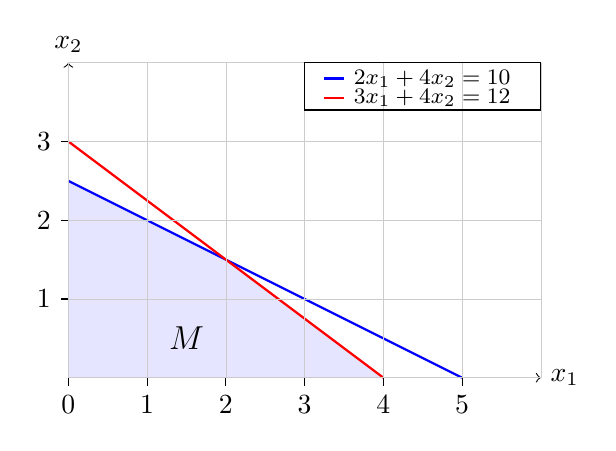
\begin{tikzpicture}[scale=1]
        \fill[blue!20,opacity=0.5]
            (0,0) -- 
            (0,2.5) -- 
            (2,1.5) -- % 
            (4,0) -- 
            (0,0);
        \node[black] at (1.5,0.5) {\large $M$};
    
        \draw[->] (0,0) -- (6,0) node[right] {$x_1$};
        \draw[->] (0,0) -- (0,4) node[above] {$x_2$};
    
        \foreach \x in {0,1,2,3,4,5} \draw (\x,0) -- (\x,-0.1) node[below] {\x};
        \foreach \y in {1,2,3} \draw (0,\y) -- (-0.1,\y) node[left] {\y};
    
        % 2x1 + 4x2 = 10  => x2 = (10 - 2x1)/4
        \draw[thick,blue] (0,2.5) -- (5,0);
    
        % 3x1 + 4x2 = 12 => x2 = (12 - 3x1)/4
        \draw[thick,red] (4,0) -- (0,3);
    
        \draw[step=1cm,gray!40,very thin] (0,0) grid (6,4);
    
        \begin{scope}[shift={(3,3.8)}, scale=0.5]
            \draw[black] (0,0.4) rectangle (6,-0.8); 
            \draw[thick,blue] (0.5,0) -- (1,0);
            \node[right] at (1,0) {\footnotesize $2x_1 + 4x_2 = 10$};
    
            \draw[thick,red] (0.5,-0.5) -- (1,-0.5);
            \node[right] at (1,-0.5) {\footnotesize $3x_1 + 4x_2 = 12$};
        \end{scope}
    \end{tikzpicture}

\columnbreak

    Graficky lze nalézt, že maximum se nabývá v bodě $(2, \frac{3}{2})^T$. Maximum je $f(2, \frac{3}{2}) = 27$.
\end{multicols}
Pokračování příkladu.

Obchodník chce od firmy koupit veškerý materiál ze skladu. Jaké ceny za materiál $X$ a $Y$ by měl firmě nabídnout, aby 
zaplatil co nejmenší částku a firmě se přesto vyplatilo materiál prodat namísto výroby výrobků?

\newpage
Tato otázka vede na úlohu:
\begin{flalign*}
    y_1& \dots \text{cena za jednotkové množství materiálu } X& \\
    y_2& \dots \text{cena za jednotkové množství materiálu } Y&
\end{flalign*}
\begin{align*}
    \text{minimalisujte } 10y_1 + 12y_2 \\
    \text{za podmínek } 2y_1 + 3y_2 &> 6, \\
    4y_1 + 4y_2 &> 10,\\
    y_1, y_2 &\geq 0. 
\end{align*}
Pozorování. Tyto dvě úlohy jsou navzájem duální.

\subsection{Zápis úlohy lineárního programování}
Je dána úloha
\begin{align*}
    \text{minimalisujte } x_1 - x_2 \\
    \text{za podmínek } 2x_1 - 3x_2 &= 5, \\
    -2 \leq x_2 &\leq 3, \\
    x_1 &\leq 0. 
\end{align*}
Zapišme úlohu v kanonickém tvaru.\\
Pomocné substituce: $y_1 = -x_1$, $x_2 = y_2 - y_3$, $y_2, y_3 \geq 0$.
\begin{align*}
    \text{minimalisujte } -y_1-y_2+y_3 \\
    \text{za podmínek } -2y_1 - 3y_2 + 3y_3 &\geq 5, \\
    2y_1 + 3y_2 - 3y_3 &\geq -5, \\
    -y_2 + y_3 &\geq -3, \\
    y_2 - y_3 &\geq -2,\\
    y_1, y_2, y_3 &\geq 0.
\end{align*}

Zapišme úlohu ve standardním tvaru.
\begin{align*}
    \text{minimalisujte } -y_1-y_2+y_3 \\
    \text{za podmínek } -2y_1 - 3y_2 + 3y_3 & = 5, \\
    y_2 - y_3 - y_4 &= -2, \\
    y_2 - y_3 + y_5 &= 3, \\
    y_1, y_2, y_3, y_4, y_5 &\geq 0.
\end{align*}

\subsection{Basický přípustný bod}\label{BPB}
Bod $x \in M$ se nazve basický přípustný bod (BPB) úlohy lineárního programování, pokud existuje $m$-prvková množina 
$B \subseteq \bc{1, \dots, n}$ taková, že 
\begin{enumerate}[(a)]
    \item $A_B$ je regulární,
    \item $x_j = 0$ pro každé $j \in \N$.
\end{enumerate}
Množina $B$ z definice BPB se nazývá přípustná báse.

\subsection{Příklad BPB}
Nechť
$A = 
    \begin{bmatrix}
        1 & 2 & 3 \\
        0 & 2 & 3    
    \end{bmatrix} 
$ a $b = 
    \begin{bmatrix}
        5 \\
        3
    \end{bmatrix}
$. Jaké jsou BPB?
\begin{itemize}
    \item $B = \bc{1,2} \dots A_B = 
    \begin{bmatrix}
        1 & 2 \\
        0 & 2
    \end{bmatrix}$. Evidentně invertibilní. \\
    $x = 
    \begin{bmatrix}
    x_1 \\
    x_2 \\
    x_3    
    \end{bmatrix} \dots \underbrace{Ax}_{A_B x_B +  A_N\underbrace{x_N}_{=0}}=b$. Tedy 
    $\left[
        \begin{array}{cc|c}
        1 & 2 & 5 \\
        0 & 2 & 3
        \end{array}
    \right]
    \rightarrow x = \frac{1}{2}
    \begin{bmatrix}
        1 \\
        3 \\
        0
    \end{bmatrix} \in M$ je BPB.
    \item $B = \bc{1,3} \dots A_B = 
    \begin{bmatrix}
        1 & 3 \\
        0 & 3
    \end{bmatrix}$. Evidentně invertibilní. \\
    Tedy 
    $\left[
        \begin{array}{cc|c}
        1 & 3 & 5 \\
        0 & 3 & 3
        \end{array}
    \right]
    \rightarrow x =
    \begin{bmatrix}
        2 \\
        0 \\
        1
    \end{bmatrix} \in M$ je BPB.
    \item $B = \bc{2,3} \dots A_B = 
    \begin{bmatrix}
        2 & 3 \\
        2 & 3
    \end{bmatrix}$. Evidentně není regulární. Žádný bod nemůže být BPB.
\end{itemize}

\subsection{Tvrzení o charakterisaci BPB}\label{charBPB}
Nechť $x \in M$. Pak $x$ je BPB právě tehdy, když $\bc{a_j \mid j \in J(x)}$ je lineárně nezávislá množina.

Důkaz.\\
\enquote{$\Rightarrow$}: $x$ je BPB $\implies$ existuje $B \subseteq \bc{1, \dots, n}$ $m$-prvková tak, že 
$\bc{a_j \mid j \in B}$ je lineárně nezávislá. Navíc $J(x) \subseteq B$, protože $J(x)$ obsahuje ty indexy, které 
odpovídají kladným komponentám a všechny komponenty indexované mimo indexy z $B$ jsou nulové. 

Tedy $\bc{a_j \mid j \in J(x)}$ je lineárně nezávislá.

\enquote{$\Leftarrow$}: Je-li $|J(x) = m|$, pak jasné ($B = J(x)$).\\
Ať $|J(x)| < m$. Z předpokladu víme $\rank(A) = m$. Pak lze $J(x)$ doplnit do $m$-prvkové množiny 
$B \subseteq \bc{1,\dots, n}$ tak, že $\bc{a_j \mid j \in B}$ je lineárně nezávislá. $\implies x$ je BPB. $\qed$

\subsection{Tvrzení, že dva různé PBP musí mít různé množiny \texorpdfstring{$B$}{B}} \label{ruzneBPB}
Pro každou $m$-prvkovou množinu $B \subseteq \bc{1, \dots, n}$ takovou, že $A_B$ je regulární, existuje nejvýše jedno 
$x \in M$ splňující $x_j = 0$ pro každé $j \in N$.

Důkaz. Sporem.

Ať $x, y \in M$ jsou různé a splňují $x_j = y_j = 0$ pro každé $j \in N$.

\[
    \begin{rcases}
        b = Ax = \sum_{j = 1}^{n} x_j a_j = \sum_{j \in B}x_j a_j = A_B x_B \\
        b = Ay = A_B y_B
    \end{rcases} A_B x_B = A_B y_B
\]
A protože $A$ je dle předpokladu regulární, tak dostaneme:
\[
    x_B = y_B \implies x = y
\]
Což je ale spor, protože $x$ a $y$ mají být různé. $\qed$

Horní hranice počtu BPB úlohy LP je tedy $\binom{n}{m}$.

\subsection{Příklad na degenerované BPB}
Nechť 
\[
    A = 
    \begin{bmatrix}
    1 & 0 & 1 & 1 \\
    1 & 1 & 0 & 1
    \end{bmatrix} \quad \text{ a } \quad b = 
    \begin{bmatrix}
        1 \\
        1
    \end{bmatrix}.
\]
Určete všechny basické přípustné body.

\begin{itemize}
    \item $B = \bc{1,2}$. Tedy $A_B = 
        \begin{bmatrix}
            1 & 0 \\
            1 & 1
        \end{bmatrix}$ je určitě regulární.\\
        Pak očividně $\begin{bmatrix}1, 0, 0, 0\end{bmatrix}^T$ je BPB s přípustnou básí $B$.
    \item $B = \bc{1,3}$. Tedy $A_B = 
        \begin{bmatrix}
            1 & 1 \\
            1 & 0
        \end{bmatrix}$ je určitě regulární.\\
        Pak $\begin{bmatrix}1, 0, 0, 0\end{bmatrix}^T$ je BPB s přípustnou básí $B$.
    \item $B = \bc{1,4}$. $A_B = 
        \begin{bmatrix}
            1 & 1 \\
            1 & 1
        \end{bmatrix}$ je singulární, tedy není přípustnou básí BPB.
    \item $B = \bc{2,3}$. Tedy $A_B = 
        \begin{bmatrix}
            0 & 1 \\
            1 & 0
        \end{bmatrix}$ je určitě regulární.\\
        Pak $\begin{bmatrix}0, 1, 1, 0\end{bmatrix}^T$ je BPB s přípustnou básí $B$.
    \item $B = \bc{2,4}$. Tedy $A_B = 
        \begin{bmatrix}
            0 & 1 \\
            1 & 1
        \end{bmatrix}$ je určitě regulární.\\
        Pak $\begin{bmatrix}0, 0, 0, 1\end{bmatrix}^T$ je BPB s přípustnou básí $B$.
    \item $B = \bc{3,4}$. Tedy $A_B = 
        \begin{bmatrix}
            1 & 1 \\
            0 & 1
        \end{bmatrix}$ je určitě regulární.\\
        Pak $\begin{bmatrix}0, 0, 0, 1\end{bmatrix}^T$ je BPB s přípustnou básí $B$.
\end{itemize}

\subsection{Příklad na souvislost BPB a krajních bodů}
Nechť
\[
    A = 
    \begin{bmatrix}
    1 & 2 & 3 \\
    0 & 2 & 3
    \end{bmatrix} \quad \text{ a } \quad b = 
    \begin{bmatrix}
        5 \\
        3
    \end{bmatrix}.
\]
$M = \bc{x \in \R^3_+ \mid Ax = b}$.

Již víme, že $x = 
\begin{bmatrix}
2 \\
0 \\
1    
\end{bmatrix}$ a $y = 
\begin{bmatrix}
    2 \\
    \frac{3}{2} \\
    0
\end{bmatrix}$ jsou BPB.

\[
    Ax = b \dots 
    \left[
        \begin{array}{ccc|c}
        1 & 2 & 3 & 5 \\
        0 & 2 & 3 & 3
        \end{array}
    \right] \sim
    \left[
        \begin{array}{ccc|c}
        1 & 0 & 0 & 2 \\
        0 & 2 & 3 & 3
        \end{array}
    \right]
\]
Tedy řešení soustavy $z = 
\begin{bmatrix}
2 \\
\frac{1}{2}(3-3t) \\
t
\end{bmatrix}, t \in \R$. Kdy je $z \in \R^3_+$?

Právě tehdy, když $t \geq 0$ a $1\geq t$, tedy $t \in [0,1]$.

\[
    z \in [x, y] \iff z = tx + (1-t)y = 
    \begin{bmatrix}
        2 \\
        \frac{3}{2} \\
        0
    \end{bmatrix} + t
    \begin{bmatrix}
        \phantom{-}0 \\
        -\frac{3}{2} \\
        \phantom{-}1
    \end{bmatrix} = 
    \begin{bmatrix}
        2 \\
        \frac{3}{2} (1-t) \\
        t
    \end{bmatrix}, t \in [0,1].
\]
Tedy $M = [x, y]$.

\subsection{Věta o souvislosti BPB a krajních bodů}
\begin{enumerate}[(a)]
    \item Nechť $x \in M$. Pak $x$ je BPB úlohy LP právě tehdy, když $x$ je krajní bod množiny $M$.
    \item $M$ je neprázdná právě tehdy, když existuje BPB úlohy LP.
\end{enumerate}

Důkaz (a).

\enquote{$\Rightarrow$}: Sporem.

Existují dva různé body $y, z \in M$ tak, že $x = \frac{y+z}{2}$. Ať $B$ je přípustná báse BPB $x$.

Pak $y_j = z_j = 0$ pro každé $j \in N$. Navíc $A_B$ je regulární dle \hyperref[BPB]{definice BPB}. Ale dle této stejné 
definice platí, že $y$ a $z$ jsou BPB s přípustnou básí $B$. Ale dle \hyperref[ruzneBPB]{tvrzení} nemohou mít dva různé
BPB stejnou přípustnou bási. $\implies y = z$, což je spor.

\enquote{$\Leftarrow$}: Sporem.

Ať $x$ není BPB. Pak z \hyperref[charBPB]{charakterisace BPB} plyne, že $\bc{a_j \mid j \in J(x)}$ je lineárně závislá 
množina.

$\rightarrow$ existují $d_j \in \R, j \in J(x)$, ne všechny nulové tak, že 
\[
    \sum_{j\in J(x)} d_j a_j = 0.
\]
Definujme $d_j = 0$ pro každé $j \in \bc{1, \dots, n} \setminus J(x)$.

Pak $A d = 0$. Odtud $A(x\pm \alpha d) = b \pm \alpha \underbrace{A d}_{=0} = b$ pro všechna $\alpha \in \R$.

Pro dostatečně malé $\alpha > 0$ je $x \pm \alpha d \geq 0$. Pro takové $\alpha$ je $x \pm \alpha d \in M$. Pak 
$x + \alpha d \not = x - \alpha d$ a navíc evidentně platí $x = \frac{(x+\alpha d) + (x - \alpha d)}{2}$. To je spor s 
tvrzením, že máme krajní bod. $\qed$

Důkaz (b). Vynecháme.

\subsection{Základní věta lineárního programování}
\begin{enumerate}[(a)]
    \item Úloha LP má řešení právě tehdy, když $M$ je neprázdná a $\langle x, c\rangle$ je zdola omezená na $M$.
    \item Má-li LP řešení, pak existuje řešení úlohy LP, které je BPB.
\end{enumerate}

\subsection{Tvrzení o množině všech řešení úlohy LP}
Množina všech řešení úlohy LP je konvexní polyedrická množina. 